\documentclass{article}
\usepackage{iclr2027_conference,times}
\input{math_commands.tex}
\usepackage{hyperref}
\usepackage{url}
\usepackage{amsmath,amssymb,amsthm}
\usepackage{graphicx}
\usepackage{booktabs}
\usepackage{multirow}
\usepackage{xcolor}
\usepackage{tikz}
\usetikzlibrary{arrows.meta,positioning,fit}
\usepackage{siunitx}

\newtheorem{proposition}{Proposition}
\newtheorem{fact}{Fact}
\newcommand{\sexec}{\sigma_{\mathrm{exec}}}
\newcommand{\schunk}{\sigma_{\mathrm{chunk}}}
\newcommand{\todo}[1]{\textcolor{red}{[#1]}}

\title{What an Action Interface Can Change:\\ An Identity, a Noise Exchange Rate,\\ and a Conditioning Cost}

\author{Anonymous authors\\ Paper under double-blind review}

% \iclrfinalcopy
\begin{document}

\maketitle

\begin{abstract}
Velocity, increment and low-pass action interfaces promise smoother execution, easier RL fine-tuning and robustness. All of them are one first-order filter, $c_t=\lambda c_{t-1}+s\,u_t$, and when the policy observes the filter state, as derivative labels require, the interface is the position policy in other coordinates: integration changes nothing about intent. What an interface can change reduces to three quantities. The target scale $s$ sets the imitation prior through label signal-to-noise. The exchange rate from policy-side exploration noise to the displacement the plant sees within one decision period sets how much exploration fine-tuning tolerates and how much actuator-drift robustness that exploration buys, along one curve for raw, low-pass and derivative interfaces; interfaces must therefore be compared at matched executed noise, and a comparison at matched policy-side noise credited one interface with 25 to 37 spurious points. Observing the previous command raises the prior by 11 to 21 points and costs 12 to 53 points of drift robustness at high noise. Smoothing intent and a trainable derivative prior are mutually exclusive.
\end{abstract}

\section{Introduction}

A learned robot policy rarely commands the plant directly. Between the network output and the actuators sits an \emph{action interface}: a position delta tracked by an operational-space controller, a velocity integrated by the controller, an increment or ``derivative'' integrated once more, or a command passed through a low-pass filter. The choice is a hidden hyperparameter of every RL fine-tuning recipe for imitation-learned policies~\citep{ren2024diffusionpolicypolicyoptimization,li2026reinforcementlearningactionchunking}, it moves fine-tuning success and deployment robustness by tens of points on the same task and pipeline, and it is credited with smoother execution~\citep{mysore2021caps,raffin2021smoothexplorationroboticreinforcement}, better-shaped exploration~\citep{eberhard2023pink,korenkevych2019autoregressive}, robustness to drift, and a safe site for deployment-time adaptation~\citep{muttaqien2026orpaonlineresidualpolicy,wagenmaker2025steeringdiffusionpolicylatent}. The evidence behind each credit is one configuration against one baseline at the same policy-side exploration noise.

This paper gives a model of what the interface can change. Write it as
\begin{equation}
c_t=\lambda\,c_{t-1}+s\,u_t,\qquad \lambda\in[0,1],\ s>0,
\label{eq:filter}
\end{equation}
with $u_t$ the policy output and $c_t$ the executed command. The raw policy is $(\lambda,s)=(0,1)$, a first-order low-pass filter is $(\alpha,1-\alpha)$, and a leaky ``derivative'' interface is any point with DC gain $s/(1-\lambda)>1$. A derivative policy is trained on demonstrations relabelled as increments, $u_t=(a_t-\lambda c_{t-1})/s$, and because the label depends on the filter state, the state $c_{t-1}$ is appended to the observation. Substituting the label into the filter gives $c_t=a_t$: \textbf{the observable-state derivative interface is the position policy in other output coordinates}, conditioned on its previous command, with its regression target rescaled by $1/s$. Integration changes nothing about the intended trajectory. The filter acts on what is \emph{added} to the output in $u$-coordinates: exploration noise, model error, adaptive corrections.

The identity fixes what an interface can buy, and the paper prices each item on a map of twelve trained configurations spanning $(\lambda,s)$, the training noise $\sigma$ and the observability of the filter state (Table~\ref{tab:points}), in the DPPO pipeline~\citep{ren2024diffusionpolicypolicyoptimization} for RL fine-tuning of diffusion policies~\citep{chi2023diffusionpolicy} on robomimic Square~\citep{mandlekar2021robomimic}. Three quantities carry every effect. The \emph{target scale} $s$ sets the imitation prior: labels at $s=1$ sit below the diffusion model's output-noise floor, and the prior improves from 49 to 58.5\% as $s$ falls from 1 to 0.3. The \emph{exchange rate} from policy-side noise $\sigma$ to the displacement the plant sees within one decision period, $\schunk$, sets the exploration fine-tuning tolerates and the actuator-drift robustness that exploration buys; raw, low-pass and derivative interfaces lie on one curve in $\schunk$, so interfaces must be compared at matched executed noise, and a comparison at matched policy-side $\sigma$ credited the derivative interface with 25 to 37 points it did not have. \emph{Conditioning on the previous command}, which the derivative labels require, raises the prior and costs drift robustness: at equal $\schunk$, observable-state policies trail unobservable ones by 12 points at $\schunk=0.12$ and by 30 to 53 points at $0.18$ to $0.26$, the shortcut-breaking pattern of causal confusion~\citep{dehaan2019causalconfusion,wen2020copycat}.

DART~\citep{laskey2017dart} and dynamics randomization~\citep{peng2018dynamicsrandomization} establish that training perturbation buys robustness. This paper establishes the coordinate in which that effect is invariant across action interfaces, shows that the interface rescales the coordinate silently, and separates it from the two other things an interface changes.

\paragraph{Contributions.}
\begin{enumerate}
\item \textbf{An identity and a decomposition} (Sec.~\ref{sec:theory}). With the filter state observed, closed-loop relabelling is an exact change of coordinates, $c_t=a_t$. Its verified corollaries: the policy output is the demonstration pre-whitened by $\lambda$, with a lag-1 autocorrelation predicted in closed form and present in the relabelled data before training; deterministic execution has the demonstrations' jerk (0.07--0.13 against 0.107), $2.8$--$3.2\times$ that of an unobservable low-pass twin at equal filter and noise; corrections applied upstream of the filter are absorbed by the policy. What remains for an interface to change is the target scale, the noise exchange rate, and whether the policy sees its last command.
\item \textbf{The exchange rate} (Sec.~\ref{sec:noise}). Fine-tuning reaches 92--99.5\% for executed chunk-scale noise $\schunk\in[0.035,0.26]$ whenever the prior is at least 38\%, and collapses at $\schunk\approx0.9$; actuator-gain-drift robustness rises with $\schunk$ for raw, low-pass and derivative interfaces (Spearman $\rho=0.74$ over eleven configurations, $0.90$ over the ten without the original interface). Five of six pre-registered robustness ranges for held-out configurations hit. Comparisons between interfaces must match $\schunk$.
\item \textbf{The conditioning cost} (Sec.~\ref{sec:cond}). At equal $\schunk$, policies that observe the filter state pay a drift penalty that is zero at $\schunk=0.035$, 12 points at $0.12$ and 30--53 points at $0.18$--$0.26$ (six of seven observable-state configurations below the unobservable reference, mean $-21$ points); the same conditioning, with the rescaled target, lifts the prior by 11--21 points. Smoothing intent and a trainable derivative prior are mutually exclusive: the filter either is observed and cannot smooth intent, or is not and has no identifiable derivative labels.
\end{enumerate}

\section{First-order action filters}
\label{sec:theory}

\subsection{Definitions}

The controller accepts a normalized command $c_t\in[-1,1]^d$ per control step (position and rotation deltas; the gripper bypasses the filter). The interface is~\eqref{eq:filter} followed by clipping to $[-1,1]$. The \emph{raw} interface is $(0,1)$. A \emph{low-pass} interface with coefficient $\alpha$ is $(\alpha,1-\alpha)$: unit DC gain, a policy trained in the position domain, the filter inserted at fine-tuning time, filter state hidden from the policy. A \emph{derivative} interface is $(\lambda,s)$ with $s/(1-\lambda)>1$; its policy is trained on demonstrations relabelled \emph{closed-loop} against the filter's own state,
\begin{equation}
u_t=\mathrm{clip}\!\big((a_t-\lambda c_{t-1})/s,\,-1,1\big),\qquad c_t=\lambda c_{t-1}+s\,u_t,
\label{eq:relabel}
\end{equation}
so that clipping errors do not accumulate. The label depends on $c_{t-1}$, which is not a function of the robot state; without access to it a diffusion prior fit the position dimensions with correlation $\approx0$ and achieved 0\% success. All derivative points therefore append $c_{t-1}$ to the observation (\emph{observable state}). Figure~\ref{fig:schematic} summarizes the two designs.

\begin{figure}[t]
\centering
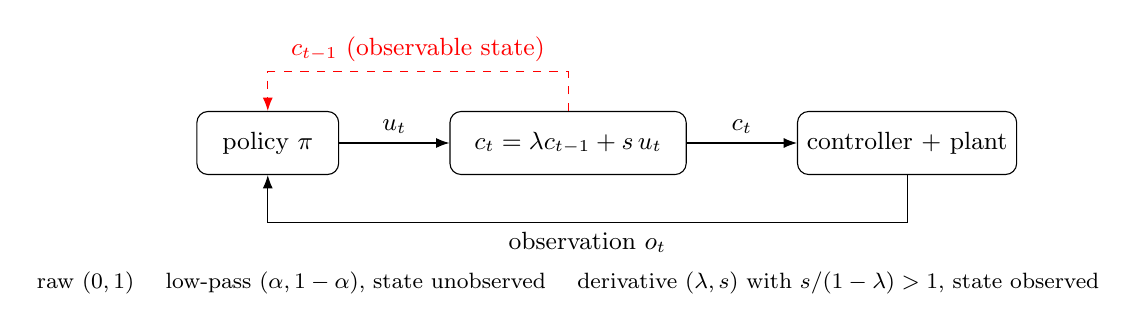
\begin{tikzpicture}[>=Latex, node distance=9mm, every node/.style={font=\small}]
\node[draw, rounded corners, minimum width=18mm, minimum height=8mm] (pi) {policy $\pi$};
\node[draw, rounded corners, right=14mm of pi, minimum width=30mm, minimum height=8mm] (f) {$c_t=\lambda c_{t-1}+s\,u_t$};
\node[draw, rounded corners, right=14mm of f, minimum width=18mm, minimum height=8mm] (plant) {controller + plant};
\draw[->] (pi) -- node[above] {$u_t$} (f);
\draw[->] (f) -- node[above] {$c_t$} (plant);
\draw[->] (plant.south) -- ++(0,-6mm) -| node[pos=0.25, below] {observation $o_t$} (pi.south);
\draw[->, dashed, red] (f.north) -- ++(0,5mm) -| node[pos=0.25, above] {\textcolor{red}{$c_{t-1}$ (observable state)}} (pi.north);
\node[below=11mm of f, align=center, font=\footnotesize] {raw $(0,1)$ \quad low-pass $(\alpha,1-\alpha)$, state unobserved \quad derivative $(\lambda,s)$ with $s/(1-\lambda)>1$, state observed};
\end{tikzpicture}
\caption{Every interface studied here is the same first-order filter. The derivative interface differs from a low-pass filter in its DC gain and in the red feedback path. With the red path present the filter is invisible to the intended trajectory (Proposition~\ref{prop:identity}); the path itself is the conditioning whose cost Sec.~\ref{sec:cond} measures.}
\label{fig:schematic}
\end{figure}

\subsection{The identity}

\begin{proposition}[Observable-state interfaces are reparameterizations]
\label{prop:identity}
Substituting~\eqref{eq:relabel} into~\eqref{eq:filter} gives $c_t=\lambda c_{t-1}+(a_t-\lambda c_{t-1})=a_t$ whenever the clip is inactive. A policy that reproduces its labels executes the demonstrated command exactly, for every $(\lambda,s)$: the derivative interface is the position policy $\pi(a_t\mid o_t,c_{t-1})$ written in the output coordinates $(a_t-\lambda c_{t-1})/s$.
\end{proposition}

\noindent Four corollaries follow.
\begin{description}
\item[(i) Intent is untouched.] The executed trajectory is the intended trajectory plus the \emph{filtered} model error. An observable-state interface is smoother than the raw policy by the amount the raw policy's model error exceeds the demonstrations' roughness, and never smoother than the demonstrations.
\item[(ii) The output is pre-whitened.] When the filter tracks the demonstration, the label is $(a_t-\lambda a_{t-1})/s$: the demonstration pre-whitened by $\lambda$. For a demonstration command with lag-1 autocorrelation $\phi$ under an AR(1) model, the label's lag-1 autocorrelation is $(\phi-\lambda)(1-\lambda\phi)/(1+\lambda^2-2\lambda\phi)$: zero at $\lambda=\phi$, negative above, positive below. This is a property of the data.
\item[(iii) Upstream corrections are disturbances.] A rescaling of $u$ changes the map from output to $c$; the policy observes $c$ and is trained to produce whatever $u$ realizes its intended $c$, so it inverts the rescaling at the next decision.
\item[(iv) Impossibility.] A filter either is observed, and then cannot smooth intent, or is not, and then the derivative labels are not identifiable and the position prior is mismatched to the filtered plant.
\end{description}
The identity leaves an interface three things to change: the scale of the regression target ($1/s$), the conditioning of the policy on $c_{t-1}$, and how perturbations added in $u$-coordinates reach the plant. Sections~\ref{sec:intent}--\ref{sec:cond} price each.

\subsection{Three facts about perturbations}

Let $\delta u_t$ be anything added to the output in $u$-coordinates and $\delta c_t$ its image on the executed command.

\begin{fact}[Spectral shaping]
\label{fact:spectrum}
For white $\delta u_t$ of variance $\sigma^2$ and $\lambda<1$, $\delta c_t$ is AR(1) with stationary standard deviation $\sexec=s\sigma/\sqrt{1-\lambda^2}$, flat below the corner frequency $\approx(1-\lambda)/2\pi$ and rolling off at exponent 2 above it; over the episode and chunk time-scales the band-averaged exponent rises from 0 at $\lambda=0$ towards 2, passing the pink-noise value $\beta\approx1$~\citep{eberhard2023pink} near $\lambda\approx0.7$. For $\lambda=1$ the variance grows as $s^2\sigma^2t$.
\end{fact}
The policy replans every $H$ steps, so the perturbation it can react to is the displacement accumulated over a chunk. For AR(1) noise this is $\schunk=\sexec\sqrt{\sum_{i,j<H}\lambda^{|i-j|}}$, which equals $2\sigma$ for white noise and $3.5$--$3.9\,\sexec$ for $\lambda\in[0.8,0.95]$ at $H=4$: at equal stationary variance, coloured noise is 1.75 to 1.9 times more visible to a policy that replans every four steps. $\schunk$ is the exchange rate of this paper: the interface sets it by $s/\sqrt{1-\lambda^2}$ at stationary scale and by a further 1.75--1.9 at chunk scale without any change to the policy-side $\sigma$.

\begin{fact}[Bounded propagation]
If $|\delta u_t|\le\Delta$ and $\lambda<1$, then $|\delta c_t|\le s\Delta/(1-\lambda)$ and $|\delta x_t|\le\|g\|_1\,s\Delta/(1-\lambda)$ for a tracking controller with impulse response $g$.
\end{fact}

\begin{fact}[Execution-space trust region]
$|c_t-c_{t-1}|\le(1-\lambda)C_{\max}+s$, independently of how far the policy parameters moved.
\end{fact}

Facts~1--3 depend on $(\lambda,s)$ only and hold identically for low-pass and derivative interfaces; by Proposition~\ref{prop:identity} they constrain perturbations. Fact~1 applies to anything injected \emph{upstream} of the filter and to nothing injected downstream, so the placement of an adaptive correction decides whether the filter protects it. With $C_{\max}=1$ the Fact~3 bound is $0.4$ at $(0.8,0.2)$ and $1.1$ at $(0.9,1.0)$: the original interface's $s=1$ made its trust region barely tighter than the raw policy's ($2$).

\section{Related work}

\paragraph{Action-space choice.} The action space matters for RL in locomotion~\citep{peng2017actionspace} and contact-rich manipulation~\citep{martinmartin2019variableimpedance}; diffusion policies were reported to prefer position over velocity control~\citep{chi2023diffusionpolicy}. These comparisons hold the policy-side noise fixed; Fact~1 shows the interface changes the executed noise silently. Our derivative prior beats the position prior because it is a position policy with previous-command conditioning and a normalized target, which reconciles the two findings.

\paragraph{Smoothness and filtered exploration.} Smoothness regularizers act on the policy~\citep{mysore2021caps}; temporally correlated exploration acts on the noise through OU processes~\citep{lillicrap2016ddpg}, state-dependent exploration~\citep{raffin2021smoothexplorationroboticreinforcement}, autoregressive policies~\citep{korenkevych2019autoregressive}, coloured noise~\citep{eberhard2023pink} or parameter-space noise~\citep{plappert2018parameternoise}; the scale and colour of action noise are known to matter~\citep{hollenstein2022actionnoise}. Action chunking and temporal ensembling~\citep{zhao2023act,li2026reinforcementlearningactionchunking} are zero-order-hold filters on both intent and noise. Proposition~\ref{prop:identity} places the derivative interface in the second family: it filters noise, not intent.

\paragraph{Noise injection and robustness.} Injecting noise during imitation~\citep{laskey2017dart} and randomizing dynamics~\citep{peng2018dynamicsrandomization} buy robustness. This paper supplies the coordinate in which the effect is invariant across action interfaces and measures the exchange rate each interface applies to it.

\paragraph{Previous-command conditioning.} Conditioning on action history invites causal confusion~\citep{dehaan2019causalconfusion} and copycat behaviour~\citep{wen2020copycat}; actuator drift is the intervention that breaks the shortcut. Section~\ref{sec:cond} measures the cost as a function of executed noise.

\paragraph{Corrections on frozen policies.} Residual policies~\citep{silver2018residual,johannink2019residual}, online residual adaptation~\citep{muttaqien2026orpaonlineresidualpolicy}, latent-noise steering~\citep{wagenmaker2025steeringdiffusionpolicylatent} and parameter-level adaptation with guarantees~\citep{oconnell2024neuralflyenablesrapidlearning,kumar2021rmarapidmotoradaptation} insert a correction between observation and actuator. Corollary~(iii) says where such a correction can go when the policy observes the filter state.

\paragraph{Evaluation methodology.} The controls of Sec.~\ref{sec:design} are an action-space instance of the ``what matters'' line in deep RL~\citep{henderson2018deeprlmatters,engstrom2020implementationmatters,andrychowicz2021whatmatters,agarwal2021precipice} and of baseline-strengthening critiques~\citep{press2024rdumbsimpleapproachquestions,dauner2023partingmisconceptionslearningbasedvehicle}.

\section{Experimental design}
\label{sec:design}

\paragraph{Pipeline.} robomimic Square (nut assembly, 300 mixed-human demonstrations)~\citep{mandlekar2021robomimic} in robosuite/MuJoCo~\citep{zhu2020robosuite}, low-dimensional observations, OSC pose control at \SI{20}{Hz}, chunks of $H=4$, 400-step episodes. Diffusion MLP priors are pre-trained for 3000 epochs (the stock position prior for raw and low-pass points; a prior on relabelled data for derivative points), then fine-tuned for 200 PPO iterations with the final-step sampling noise $\sigma$ as exploration parameter~\citep{ren2024diffusionpolicypolicyoptimization}. Training seed 42 for all points; seeds 43--46 additionally for the two principal arms.

\paragraph{The map.} Table~\ref{tab:points} lists twelve configurations plus two collapsed pilot points. The $(0.8,0.2)$ filter appears as a $\{\text{stock prior, unobserved}\}\times\{\sigma=0.03,0.10\}$ pair (B, F4) and a $\{\text{retrained, observed}\}\times\{\sigma=0.03,0.10\}$ pair (F5, F7), which is the cleanest test of the conditioning cost; F1 vs E4 varies $s$ at fixed $\lambda$; F2 varies $\lambda$ at fixed $s$; F6 is F1's prior at a higher $\sigma$. Runs that separate previous-command conditioning from retraining and from target scale are listed with their predictions in Appendix~\ref{app:planned}.

\paragraph{Axes.} (1) \emph{Prior}: success of the pre-trained prior through the interface before RL. (2) \emph{Trainability}: success after 200 iterations. (3) \emph{Smoothness}: mean executed jerk and maximum per-step change of the executed command on deterministic rollouts. (4) \emph{Robustness}: frozen success under actuator gain $\times0.7$ and under a two-step control delay. (5) \emph{Signal and adaptation}: correlation of free-motion tracking residuals with the command, recovery of a residual-driven gain compensation, and its cost when fooled by a delay. Axes 3--5 use three evaluation seeds $\times100$ episodes per cell.

\paragraph{Controls.} (C1) Compare against the raw policy at the same $\schunk$, to isolate the interface, and against the raw policy at its best $\sigma$, to measure value; the two answer different questions. (C2) Include a unit-DC-gain filter at the same Fact~3 bound with the filter state hidden. (C3) A proposed mechanism comes with a measurement that can refute it (Appendix~\ref{app:casestudy}). (C4) Perturb and adapt on both sides of the filter. Omitting C1 reverses the conclusion on three of the five axes (Appendix~\ref{app:casestudy}).

\begin{table}[t]
\centering
\caption{The map. $\schunk$: executed displacement noise within one $H=4$ chunk ($\lambda=1$: random-walk positions summed over the chunk). Prior and final success from training seed~42; deployment columns are means over three evaluation seeds $\times100$ episodes. Obs.: filter state observed by the policy. P3: Fact~3 bound $(1-\lambda)+s$. E3 and C are pilot configurations with training curves only.}
\label{tab:points}
\small
\setlength{\tabcolsep}{3.3pt}
\begin{tabular}{l ccc c c | cc | cc | cc | ccc}
\toprule
& $\lambda$ & $s$ & $\sigma$ & Obs. & $\schunk$ & Prior & Final & Jerk & Max step (P3) & Gain$\times$.7 & Delay 2 & Calib.\ $\rho$ & Recover & Fooled \\
\midrule
F4 & .8   & .2  & .03 & no  & .035 & 23.5 & 77.5 & .03 & .14 (0.4) & 1.0  & 64.7 & .80 & +39.7 & $-$18.3 \\
F5 & .8   & .2  & .03 & yes & .035 & 59.5 & 94.0 & .07 & .26 (0.4) & 4.0  & 73.3 & .94 & +79.0 & $-$5.7 \\
E5 & 0    & 1.0 & .03 & --  & .060 & 38.0 & 93.0 & .16 & .67 (2.0) & 3.7  & 80.0 & .75 & +40.7 & $-$19.3 \\
F1 & .9   & .3  & .03 & yes & .078 & 58.5 & 94.0 & .07 & .30 (0.4) & 12.0 & 74.7 & .89 & +73.7 & +0.7 \\
B  & .8   & .2  & .10 & no  & .117 & 23.5 & 96.0 & .03 & .20 (0.4) & 41.0 & 87.0 & .93 & +55.7 & $-$5.3 \\
F7 & .8   & .2  & .10 & yes & .117 & 59.5 & 99.5 & .10 & .29 (0.4) & 28.7 & 86.7 & .73 & +19.7 & $-$23.3 \\
F2 & .7   & 1.0 & .03 & yes & .138 & 54.0 & 98.0 & .11 & .60 (1.3) & 38.7 & 80.0 & .93 & +58.7 & $-$21.3 \\
E1 & 1.0  & 1.0 & .03 & yes & .164 & 43.5 & 92.0 & .12 & .76 (1.0) & 45.3 & 83.0 & -- & -- & -- \\
F6 & .9   & .3  & .07 & yes & .181 & 58.5 & 99.5 & .09 & .33 (0.4) & 38.3 & 67.3 & .90 & +56.3 & +2.3 \\
F3 & .95  & .5  & .03 & yes & .186 & 59.5 & 99.0 & .10 & .43 (0.55) & 45.7 & 84.0 & .85 & +48.7 & $-$11.0 \\
A  & 0    & 1.0 & .10 & --  & .200 & 38.0 & 99.5 & .17 & .68 (2.0) & 81.3 & 91.0 & .81 & +17.0 & $-$39.3 \\
E4 & .9   & 1.0 & .03 & yes & .258 & 49.0 & 95.0 & .13 & .79 (1.1) & 28.3 & 87.3 & .75 & +62.7 & $-$11.0 \\
\midrule
C  & 1.0  & 1.0 & .10 & yes & .55  & 43.5 & 24.5 & \multicolumn{7}{l}{pilot: pure integrator, collapsed} \\
E3 & .9   & 1.0 & .10 & yes & .86  & 49.0 & 12.5 & \multicolumn{7}{l}{pilot: leaky interface at the raw policy's $\sigma$, collapsed} \\
\bottomrule
\end{tabular}
\end{table}

\section{Results I: intent, prior and target scale}
\label{sec:intent}

\paragraph{The prior is set by conditioning and target scale.} Every derivative prior beats the stock prior (49.0--59.5\% against 38.0\%), and the gain grows as $s$ shrinks: at $\lambda=0.9$, $s=1.0\to0.3$ raises the prior from 49.0 to 58.5\%; at $s=1$, $\lambda=0.9\to0.7$ from 49.0 to 54.0\%. With $s=1$ the labels~\eqref{eq:relabel} have mean magnitude $|u|\approx0.07$ in the dataset, below the diffusion model's output-noise floor in normalized units; with $s=0.3$ they fill the range while clipping fewer than 1\% of steps. This is target normalization applied where it is easy to forget, and it applies to any generative policy with a fixed output-noise floor. DC gain is irrelevant: the low-pass filter $(0.8,0.2)$ with a retrained, observable-state prior (F5) reaches 59.5\%, the same as the best derivative point, while the same filter with the stock prior starts at 23.5\%. The $\lambda=0$ corner points of Appendix~\ref{app:planned} separate the conditioning and scaling terms.

\paragraph{Deterministic execution has the demonstrations' smoothness.} The maximum per-step change of the executed command follows the Fact~3 bound across all twelve points (Table~\ref{tab:points}). Within a bound, points split by observability (Table~\ref{tab:white}). The demonstrations have lag-1 autocorrelation $\phi=0.91$, band-averaged spectral exponent $1.93$ and jerk $0.107$. Policies that do not observe the filter state (B, F4) output commands as smooth as the raw policy's ($\mathrm{ac}_1\approx0.8$) and the filter smooths them further: executed jerk $0.026$--$0.032$, exponent $\approx3$. Policies that observe the filter state output white or anti-correlated commands ($\mathrm{ac}_1$ from $-0.14$ to $0.40$); their executed jerk is $2.8$--$3.2\times$ that of the unobservable twin at the same filter and $\sigma$ (F4$\to$F5: $0.026\to0.074$; B$\to$F7: $0.032\to0.101$) and lands on the demonstrations' value ($0.07$--$0.13$ against $0.107$), as does the exponent ($1.8$--$2.25$ against $1.93$). The raw policy is jerkier than the demonstrations ($0.16$--$0.18$) because its model error is executed unfiltered; the observable-state interface removes that excess and nothing more, as corollary~(i) requires.

\paragraph{The whitening is in the data.} Corollary~(ii) predicts the sign of $\mathrm{ac}_1(u)$ from $\phi$ and $\lambda$: with $\phi=0.91$, labels are nearly white at $\lambda\approx0.9$, negative above and positive below. The relabelled datasets have $\mathrm{ac}_1(u)=-0.08$ at $\lambda=0.9$, $-0.14$ at $0.95$, $+0.24$ at $0.8$ and $+0.35$ at $0.7$ (AR(1) prediction $+0.35$), before any training; the fine-tuned policies reproduce them ($-0.14$, $-0.11$, $+0.25$--$0.31$, $+0.40$). The filter's shaping is visible where the identity says it should be, on perturbations: in stochastic rollouts E4's executed spectral exponent is $2.1$--$2.5$ against $0.9$ for its raw twin.

\begin{table}[t]
\centering
\caption{Command statistics on deterministic no-drift rollouts (position dimensions, three evaluation seeds) and in the demonstrations. $\mathrm{ac}_1$: lag-1 autocorrelation; $\beta$: band-averaged spectral exponent.}
\label{tab:white}
\small
\begin{tabular}{l l cc c c c}
\toprule
& State & $\mathrm{ac}_1(u)$ & $\mathrm{ac}_1(c)$ & sign flips & jerk & $\beta_c$ \\
\midrule
demonstrations & -- & -- & .91 & -- & .107 & 1.93 \\
A (raw, $\sigma$=.10) & -- & .80 & .80 & .59 & .175 & 1.48 \\
E5 (raw, $\sigma$=.03) & -- & .77 & .77 & .60 & .161 & 1.76 \\
B (.8,.2,$\sigma$=.10) & unobserved & .81 & .99 & .61 & .032 & 3.04 \\
F4 (.8,.2,$\sigma$=.03) & unobserved & .78 & .99 & .61 & .026 & 2.85 \\
F5 (.8,.2,$\sigma$=.03) & observed & .31 & .96 & .70 & .074 & 1.98 \\
F7 (.8,.2,$\sigma$=.10) & observed & .25 & .96 & .70 & .101 & 2.25 \\
E4 (.9,1,$\sigma$=.03) & observed & $-$.14 & .93 & .71 & .134 & 1.83 \\
F1 (.9,.3,$\sigma$=.03) & observed & $-$.11 & .95 & .73 & .073 & 2.08 \\
F6 (.9,.3,$\sigma$=.07) & observed & .03 & .96 & .72 & .086 & 2.14 \\
F2 (.7,1,$\sigma$=.03) & observed & .40 & .94 & .67 & .115 & 2.01 \\
F3 (.95,.5,$\sigma$=.03) & observed & $-$.11 & .94 & .71 & .098 & 1.78 \\
\bottomrule
\end{tabular}
\end{table}

\begin{figure}[t]
\centering
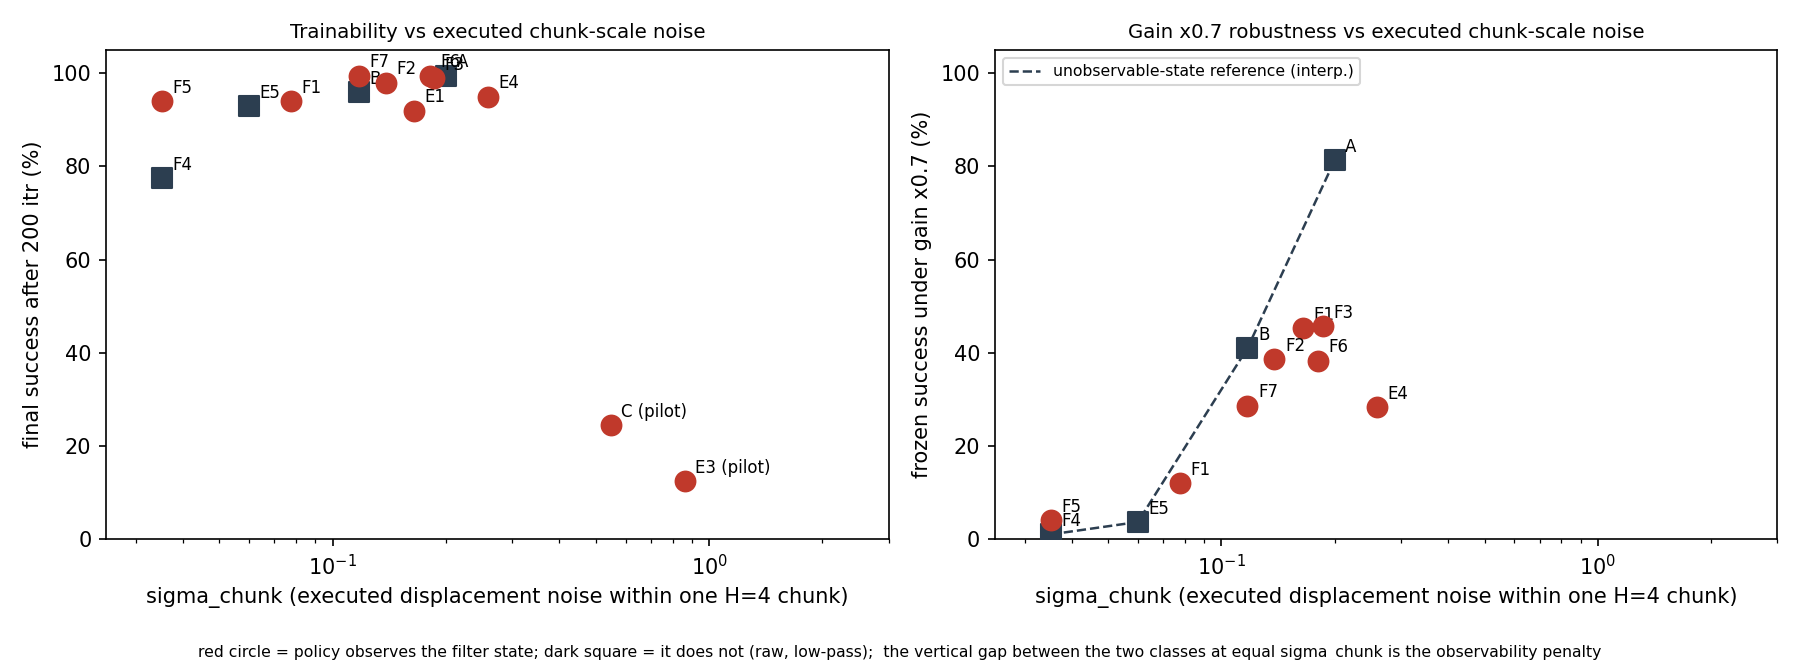
\includegraphics[width=\textwidth]{figures/DS_h9_chunk.png}
\caption{Trainability (left) and actuator-gain-drift robustness (right) against the executed chunk-scale noise $\schunk$ (log scale). Red circles: the policy observes the filter state; dark squares: it does not (raw, low-pass). Left: a plateau over $\schunk\in[0.035,0.26]$ with a prior-dependent low edge (F4 against F5 at equal noise) and a collapse near $0.9$. Right: unobservable-state points rise along one curve; observable-state points fall increasingly below it as $\schunk$ grows. The vertical gap at equal $\schunk$ is the conditioning cost of Sec.~\ref{sec:cond}.}
\label{fig:h9}
\end{figure}

\section{Results II: the noise exchange rate}
\label{sec:noise}

\paragraph{Trainability is a plateau in executed noise with a prior-dependent edge.} Fine-tuning reaches 92--99.5\% for every configuration with $\schunk\in[0.035,0.26]$ whose prior is at least 38\% (Fig.~\ref{fig:h9}, left). At the low edge the prior decides: at $\schunk=0.035$ the mismatched stock prior stalls at 77.5\% (F4) while the retrained, observable-state prior on the same filter and $\sigma$ reaches 94.0\% (F5). At the high edge the noise decides: the leaky interface fine-tuned at the raw policy's $\sigma=0.10$ ($\schunk\approx0.86$) collapses to 12.5\%, and a pure integrator at the same $\sigma$ to 24.5\%. The filter's noise gain therefore sets the usable $\sigma$: a low-pass attenuates variance by $(1-\alpha)/(1+\alpha)=0.11$ and under-explores at $\sigma=0.03$; a leaky integrator with $s=1$ amplifies it by $5.3$ and over-explores at $\sigma=0.10$. The original interface at $\sigma=0.03$ sits near the plateau's right end; over five training seeds its final success is $92.5\pm8.5\%$ (one seed at 77.5\%) against $92.1\pm1.3\%$ for its raw twin.

\paragraph{Actuator-gain-drift robustness rises with executed noise along one curve.} Under a 30\% actuator-gain loss, frozen success spans $1$--$81\%$ and is ordered by executed noise (Fig.~\ref{fig:h9}, right): Spearman $\rho=0.74$ against $\schunk$ over the eleven stationary configurations, $0.90$ over the ten without E4. Raw, low-pass and derivative points share the rising part of the curve: F4, F5, E5, F1, B and F2 read 1.0, 4.0, 3.7, 12.0, 41.0 and 38.7\% at $\schunk$ from $0.035$ to $0.14$. The chunk-scale form orders two pairs that stationary variance misorders: the raw policy at $\sigma=0.03$ (E5, $\sexec=0.030$) is as fragile as the $\sigma=0.03$ low-pass points ($3.7$ against $1$--$4\%$) although its stationary noise is three times theirs, because white noise of standard deviation $0.03$ accumulates to only $0.06$ within one decision period, whereas the same variance through a $\lambda=0.8$ filter accumulates to $0.12$ (B: 41\%); the $H$-sweep at fixed $\sexec$ is the pre-registered discriminating test (Appendix~\ref{app:planned}). Five of six robustness ranges pre-registered for held-out configurations hit (Appendix~\ref{app:prereg}); the miss is F7, the observable-state twin of B, and it is explained in Sec.~\ref{sec:cond}.

\paragraph{The rule.} A comparison between action interfaces at equal policy-side $\sigma$ compares unequal exploration. The original interface at $\sigma=0.03$ ($\schunk=0.26$) against the raw policy at the same $\sigma$ ($\schunk=0.06$) read $28.3$ against $3.7\%$ under gain drift and $+29$ points under observation noise, an advantage of 25 to 37 points that the map attributes to the noise the interface added, not to the interface: the raw policy at $\schunk=0.20$ reads 81.3\%. Interfaces must be compared at matched $\schunk$.

\paragraph{Delay robustness does not follow executed noise.} Success under a two-step control delay, in $\schunk$ order, is 64.7, 73.3, 80.0, 74.7, 87.0, 86.7, 80.0, 83.0, 67.3, 84.0, 91.0, 87.3\% (Table~\ref{tab:points}). Training noise perturbs displacement, not timing; the mediation covers perturbations in the span of the training perturbation. Among the $\sigma=0.03$ derivative points delay robustness rises with $s$ (73--75\% at $s\le0.3$, 84\% at $0.5$, 80--87\% at $1$) and falls when $\sigma$ is raised (F6: 67\%); a smaller $s$ makes the policy output larger and more feedback-dependent, and a delay corrupts that feedback.

\section{Results III: the conditioning cost}
\label{sec:cond}

\paragraph{At equal executed noise, observing the filter state costs drift robustness.} Take the unobservable-state points as the reference curve (F4, E5, B, A at $\schunk$ 0.035, 0.060, 0.117, 0.200) and read each observable-state point against it at its own $\schunk$ (Fig.~\ref{fig:h9}, right). The residuals are $+3$ (F5, 0.035), $-6$ (F1, 0.078), $-12$ (F7, 0.117), $-15$ (F2, 0.138), $-35$ (F6, 0.181), $-30$ (F3, 0.186) and $-53$ points (E4, 0.258): six of seven negative, mean $-21$, and growing with $\schunk$. The cleanest pair is B against F7, identical in $\lambda$, $s$, $\sigma$ and $\schunk$ and differing only in a retrained prior and the observed $c_{t-1}$: $41.0$ against $28.7\%$. The penalty is stable across training seeds: five seeds put E4 at $25.9\pm7.5\%$ and E5 at $4.3\pm2.7\%$. It is not prior quality (F5 and F6 carry the best priors on the map and pay $+3$ and $-35$), and it is not noise scale or colour (both metrics leave it). A policy that observes $c_{t-1}$ can fit the demonstrations by tracking its own command history instead of the state~\citep{wen2020copycat}; a gain change breaks exactly that shortcut, and the more exploration the policy saw during fine-tuning, the more of its robustness it stood to gain from the state it was not reading. On the current map observability is confounded with retraining on relabelled data, because derivative labels are not identifiable without $c_{t-1}$; the run that separates them, the raw policy with $c_{t-1}$ appended to its observation at $\sigma=0.10$, is in progress (Appendix~\ref{app:planned}).

\paragraph{The same conditioning buys the prior.} The conditioned, rescaled prior is 11 to 21 points above the stock prior (49.0--59.5 against 38.0\%) and 36 points above the stock prior through a filter it was not trained for (23.5\%). The map thus prices the previous command in both directions: a better start and a worse response to the one deployment shift that changes the meaning of the command it conditions on.

\paragraph{Where a correction is applied decides whether the filter protects it.} We estimate the actuator gain ratio $\hat g$ from free-motion tracking residuals and apply $1/\hat g$ with a dead-band trigger (Appendix~\ref{app:estimator}). Applied \emph{downstream}, on the executed command, the same estimator recovers every arm---raw $\sigma=0.10$ from 81 to 99\%, the interface from 28 to 91\%, the low-pass from 41 to 97\%---and measures the policy's closed-loop tolerance to gain error. Applied \emph{upstream}, on the policy output where Fact~1 applies, the correction recovers the low-pass arm as well as downstream does ($92$--$93\%$ against $94$--$97\%$), and injected white adaptation noise of relative standard deviation $0.5$ raises executed jerk by $1.40\times$ against $6.11\times$ downstream. On the observable-state interface the same upstream correction recovers nothing ($27$--$36\%$ against $87$--$91\%$ downstream) and makes execution jerkier ($1.7$--$2.3\times$): the policy regulates the $c$ it observes and undoes the scaling at the next decision, as corollary~(iii) predicts (Fig.~\ref{fig:upstream}). For an observable-state interface the protected adaptation site does not exist. Zero-mean adaptation noise barely affects success for any arm ($\le6$~points at relative std $0.5$); bias does, and bias is placement-invariant.

\paragraph{Signal quality follows command colour.} The calibration correlation of the tracking residual is highest for the unobservable low-pass ($0.93$) and for the observable point with the smoothest output (F5, $0.94$), and lowest for the whitened E4, E5 and F7 ($0.73$--$0.75$).

\begin{figure}[t]
\centering
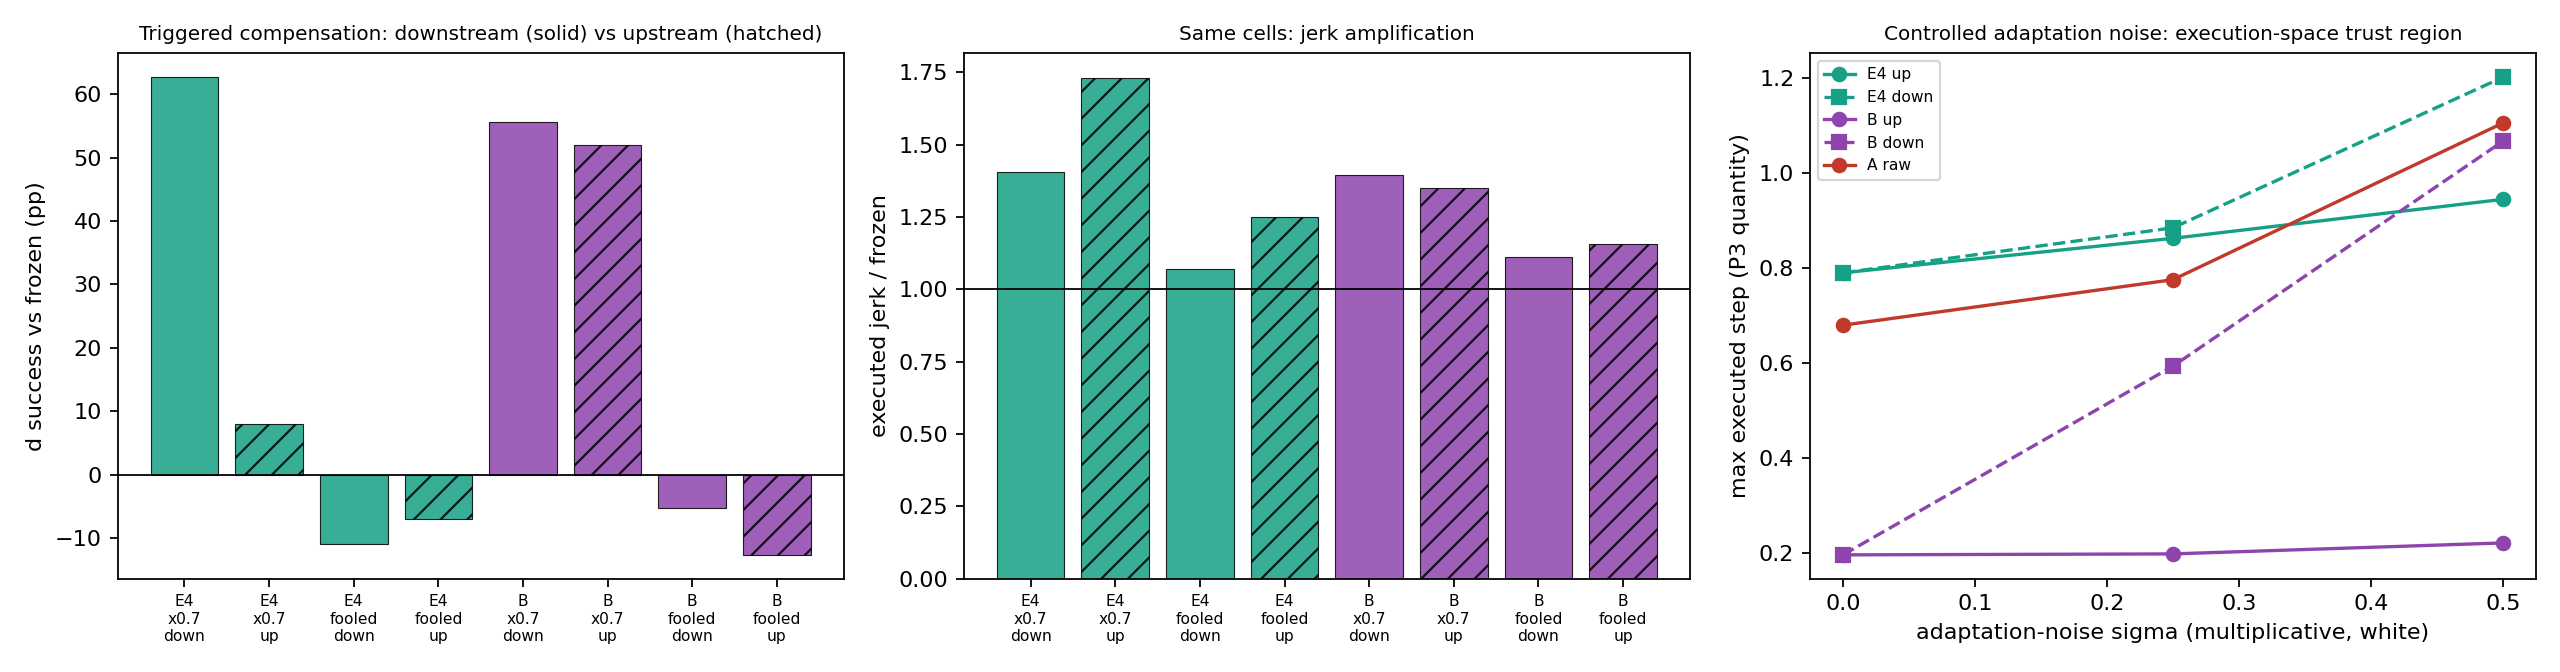
\includegraphics[width=\textwidth]{figures/P1_upstream.png}
\caption{Placement of an adaptive correction. Left/centre: triggered gain compensation applied downstream (solid) versus upstream (hatched) of the filter, under gain $\times0.7$ and under an estimator fooled by a delay; on the unobservable low-pass (B) both placements work, on the observable-state interface (E4) only downstream does. Right: maximum executed step under injected white adaptation noise; the low-pass with upstream injection stays within its Fact~3 bound.}
\label{fig:upstream}
\end{figure}

\section{What this changes for action-space design}
\label{sec:rules}

\begin{enumerate}
\item \textbf{Match executed noise, not $\sigma$.} Report $\schunk$ and match it; a comparison at equal policy-side noise compares unequal exploration and credited one interface with 25--37 points here.
\item \textbf{Choose smoothing \emph{or} a derivative prior.} An unobserved filter smooths intent and cannot be given identifiable derivative labels; an observed filter can, is a reparameterization of the position policy, and smooths only perturbations. Claims of smoother execution are checked on deterministic rollouts against an unobserved low-pass of the same Fact~3 bound.
\item \textbf{Normalize derivative targets.} $s$ sets label signal-to-noise against the generative model's output-noise floor; $s=1$ in normalized units was the single worst choice in the original interface.
\item \textbf{Price the previous command.} Conditioning on $c_{t-1}$ lifts the prior and costs actuator-drift robustness that grows with executed noise; test for it with the state hidden during behaviour cloning.
\item \textbf{Adapt downstream or not at all} when the policy sees the filter; the protected upstream site is absorbed.
\end{enumerate}
Rules~1 and~3 applied to the original interface give F6 $=(0.9,0.3)$ at $\sigma=0.07$: prior $+9.5$ points, final $99.5\%$, gain-drift robustness $+10$, maximum step $0.33$ against $0.79$, misadaptation cost $+2$ against $-11$ points, and $20$ points less delay robustness ($67$ against $87\%$). At nearly matched executed noise ($\schunk$ 0.18 against 0.20) it trails the raw policy by 43 points on gain-drift robustness and 24 on delay; the gap is the conditioning cost of Sec.~\ref{sec:cond}.

\section{Limitations}

One task (quasi-static insertion), one simulator, one RL algorithm, low-dimensional observations, and a single training seed for most configurations (five for the two principal arms). Drift robustness is measured for actuator gain; delay robustness follows a different order and is reported as such. Observability and retraining on relabelled data are confounded on the current map; the run that separates them is listed in Appendix~\ref{app:planned}. Tasks in which smoothness is a constraint rather than a preference may reward filtered interfaces differently; by corollary~(iv) the candidate there is the unobserved low-pass.

\section{Conclusion}

Derivative, velocity and low-pass action interfaces are one first-order filter. When the policy can see the filter's state, which it must for derivative labels to be learnable, the interface is the position policy in other coordinates, and what it can change reduces to the scale of its target, the exchange rate from exploration noise to executed displacement, and the conditioning on its last command. The map prices each: a prior gain of 11--21 points, a robustness curve shared by every interface in the executed-noise coordinate, and a drift penalty of 12--53 points for the conditioning at high noise. The map, the identity and the four controls give the next action-space proposal a null hypothesis to beat and one number to match.

\subsubsection*{Reproducibility statement}
Configurations, wrappers, the drift and misadaptation suites, and all rollout statistics are released at \todo{URL}. Appendix~\ref{app:prereg} lists the pre-registered predictions and the miss.

\bibliography{refs}
\bibliographystyle{iclr2027_conference}

\appendix

\section{Case study: what a matched-$\sigma$ comparison credited to the interface}
\label{app:casestudy}

A pilot compared the leaky interface $(0.9,1.0)$ fine-tuned at $\sigma=0.03$ against the raw policy fine-tuned at the same $\sigma$, because at $\sigma=0.10$ the interface collapsed (12.5\%). Against that twin the interface was $+25$ to $+37$~points more robust to actuator-gain drift and $+29$~points to observation noise, and a residual-driven gain compensation recovered the interface from 28 to 91\% while recovering the twin only to 44\% and destroying it under no drift ($-48$~points); integral action was proposed as the mechanism. Three controls settled the account. The raw policy at its default $\sigma=0.10$ is more robust than any interface configuration (81\% under gain $\times0.7$) and uses the same compensation perfectly (99\%, misadaptation cost $-0.3$~points): the twin was a low-noise policy, and the interface's $\schunk$ (0.26) was four times its twin's (0.06). The compensation ratio, executed magnitude under drift over executed magnitude without, was $0.66$ at gain $0.7$ for interface and raw alike, and the policy output was unchanged: no integral action occurred. The compensation had been applied downstream of the integrator, so Fact~2 never applied; applied upstream it was absorbed (corollary~(iii)). A procedural lesson: a delay-aware estimator whose history buffer was reset each episode produced a plausible ``fixes the negative control, costs 20 points'' result that was an artefact; new estimator paths are now checked against the old one on the no-drift condition before entering a drift grid.

\section{Pre-registered predictions}
\label{app:prereg}

Ranges for actuator-gain-drift success ($\times0.7$, frozen, three evaluation seeds) were written from the $\sexec$ trend of the first seven configurations before the held-out configurations were evaluated.

\begin{center}\small
\begin{tabular}{l c c c c}
\toprule
Configuration & $\sexec$ & Predicted range & Observed & Outcome \\
\midrule
F1 $(0.9,0.3,\sigma\,.03)$ & .021 & 5--15 & 12.0 & hit \\
F2 $(0.7,1.0,\sigma\,.03)$ & .042 & 25--40 & 38.7 & hit \\
F3 $(0.95,0.5,\sigma\,.03)$ & .048 & 30--45 & 45.7 & edge (+0.7) \\
F5 $(0.8,0.2,\sigma\,.03)$, observed & .010 & $\le5$ (alt.\ hypothesis: 8--15) & 4.0 & hit \\
F6 $(0.9,0.3,\sigma\,.07)$ & .048 & 30--45 (alt.\ hypothesis: $\ge50$) & 38.3 & hit \\
F7 $(0.8,0.2,\sigma\,.10)$, observed & .033 & 36--46 (as B) & 28.7 & miss ($-12$: the conditioning cost) \\
\bottomrule
\end{tabular}
\end{center}
The alternative hypothesis tested with F5 and F6 was that prior quality raises drift robustness; both landed in the noise-only range, and the hypothesis was retired.

\section{Estimator and misadaptation suite}
\label{app:estimator}
The nominal map $K$ from executed position command to end-effector displacement is calibrated per policy on no-drift rollouts (its effective value depends on the command autocorrelation because the controller lags by more than one step). At deployment, free-motion steps (gripper open, $|c|>0.15$) enter a sliding-window least-squares estimate of the gain ratio $\hat g$ (window 120, clipped to $[0.6,1.5]$); the triggered variant compensates only when $|\hat g-1|>0.15$ and exceeds twice its standard error, with hysteresis at $0.08$. The misadaptation suite comprises: no drift with the estimator active; a two-step delay, which the estimator misreads as $\hat g\approx0.65$--$0.85$; controlled wrong compensation (executed gain $\times1.2$--$1.6$ on frozen policies); and white multiplicative adaptation noise $(1+\varepsilon_t)$, $\varepsilon_t\sim\mathcal N(0,\sigma_\varepsilon)$, injected upstream or downstream of the filter.

\section{Runs in progress and their predictions}
\label{app:planned}
\begin{itemize}
\item \textbf{Conditioning alone.} The raw policy with $c_{t-1}$ appended to its observation ($\lambda=0$, $s=1$, retrained), fine-tuned at $\sigma=0.10$ ($\schunk=0.20$, as A). Prediction under the conditioning-cost hypothesis: gain-drift success falls from A's 81\% toward 40\%; under the retraining hypothesis it stays near 81\%. Its unobserved twin (the stock labels retrained on our pipeline, $\sigma=0.10$) controls for retraining.
\item \textbf{Top of the unobservable curve.} The raw policy at $\sigma=0.13$ ($\schunk=0.26$, as E4) and the unobserved low-pass $(0.8,0.2)$ at $\sigma=0.17$ ($\schunk=0.20$, as A). Prediction: both at or above 75\% under gain drift.
\item \textbf{$\lambda=0$ corner points} ($(0,1)$ and $(0,0.6)$, each with and without the observed previous command; behaviour cloning only). Prediction: conditioning accounts for most of the prior gain, target scale for a smaller term, retraining alone reproduces the stock prior.
\item \textbf{Chunk length} $H\in\{1,4,8\}$ at fixed $\sexec$: the $\schunk$ ordering should tighten and the $\sexec$ ordering should not.
\item \textbf{History dropout} during behaviour cloning of the observable-state points: the penalty should shrink if it is causal confusion.
\item \textbf{A second task} with different contact structure (robomimic Transport).
\end{itemize}

\end{document}
